\documentclass{article}
\usepackage[utf8]{inputenc}
\usepackage{amssymb}
\usepackage{enumitem}

\usepackage{minted}
\usepackage{xcolor}
\usemintedstyle{borland}
\definecolor{LightGray}{gray}{0.9}

\usepackage{natbib}
\usepackage{graphicx}

\usepackage{geometry}
 \geometry{
 a4paper,
 total={170mm,257mm},
 left=20mm,
 top=20mm,
 }


\title{Computer Security(CSE-565) - Homework 2}
\author{ATRAYEE NAG (PERSON\# \textbf{50288651})}
\date{September 2018}


\begin{document}

\maketitle

\section{Problem 1}
\textbf{To facilitate learning about how encryption modes work, this question asks you to derive formulas for encryption and decryption in the CFB and OFB modes. In particular, the lecture presented formulas for computing cipherblocks from plaintext and plaintext from cipherblocks for almost all modes of operation including CFB. For this question, derive similar encryption and decryption formulas for the CFB mode used as a stream cipher with r-bit messages (r $<$ n). You can use notation $S_r$(a) employed in the textbook to denote the first (most significant) r bits of a. Also use notation $\|$ to denote concatenation (i.e., a$\|$b means b appended to the end of a).
Repeat the exercise for the OFB mode used as a stream cipher with r-bit messages.}

\bigskip
\textbf{CFB Model}
\begin{figure}[h!]
\centering
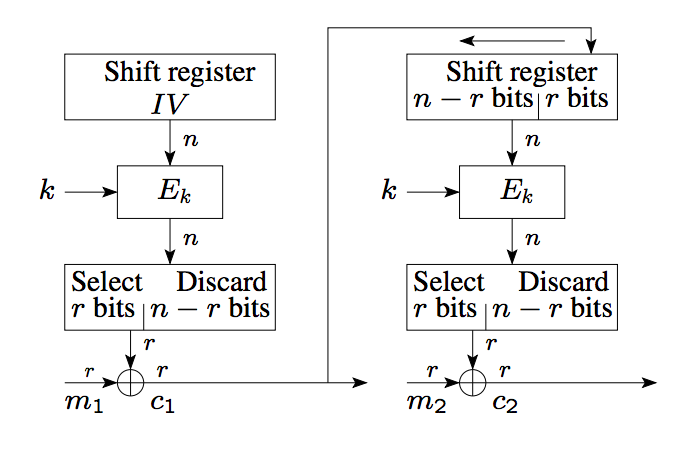
\includegraphics[scale=0.5]{CFB_mode.png}
\caption{CFB Model for Encryption}
\label{fig:aesni_output_in_c}
\end{figure}
\begin{itemize}
\item The input to the encryption function is a n-bit shift register that is initially set to some initialization vector IV.

\item The Shift register is encrypted by the secret key k through the encryption function $E_k$ and the output is denoted as $E_k$(IV) which is also of n bits.

\item The leftmost (most significant) r bits of the output $S_r$($E_k$(IV)) of the encryption function are XORed with the first unit of plaintext $m_1$ which is of r bits to produce the first unit of ciphertext $c_1$ also r bits, which is then transmitted. 
$c_1$ = $S_r$($E_k$($IV_1$)) $\oplus$ $m_1$

\item The contents of the shift register are left-shifted by r bits and $c_1$ is placed
in the rightmost (least significant) r bits of the shift register i.e. concatenated with it to create the new IV for the next iteration of encryption. Therefore $IV_2$ = ($IV_1$ $\ll$ r) $\|$ $c_1$)

The final equation stands as:

$c_1$ = $S_r$($E_k$($IV_1$)) $\oplus$ $m_1$ , $IV_2$ = ($IV_1$ $\ll$ r) $\|$ $c_1$)

By generalizing the \textbf{encryption} formula we have:

$c_i$ = $S_r$($E_k$($IV_i$)) $\oplus$ $m_i$ , $IV_i+1$ = ($IV_i$ $\ll$ r) $\|$ $c_i$)

From above, we can conclude the formula for the \textbf{decryption} algorithm is as below considering XOR of XOR is XOR function :

$m_i$ = $S_r$($E_k$($IV_i$)) $\oplus$ $c_i$ , $IV_i+1$ = ($IV_i$ $\ll$ r) $\|$ $c_i$)

\end{itemize}


\bigskip
\textbf{OFB Model}
\begin{figure}[h!]
\centering
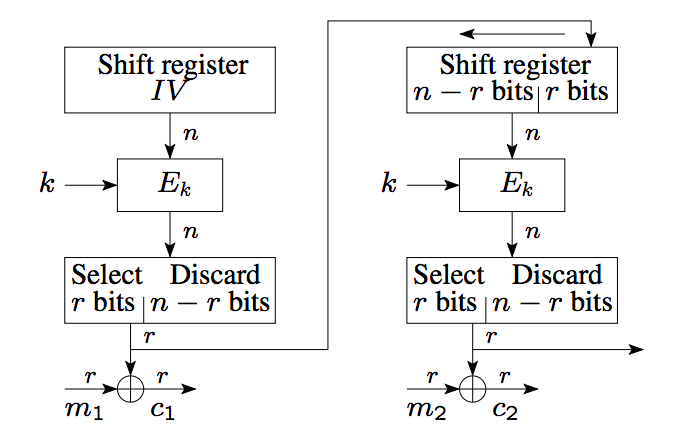
\includegraphics[scale=0.5]{OFB_mode.png}
\caption{OFB Model for Encryption}
\label{fig:aesni_output_in_c}
\end{figure}
\begin{itemize}
\item The input to the encryption function is a n-bit shift register that is initially set to some initialization vector IV.

\item The Shift register is encrypted by the secret key k through the encryption function $E_k$ and the output is denoted as $E_k$(IV) which is also of n bits.

\item The leftmost (most significant) r bits of the output $S_r$($E_k$(IV)) of the encryption function are XORed with the first unit of plaintext $m_1$ which is of r bits to produce the first unit of ciphertext $c_1$ also r bits. 
$c_1$ = $S_r$($E_k$($IV_1$)) $\oplus$ $m_1$

\item The contents of the shift register are left-shifted by r bits and the leftmost (most significant) r bits of the output $S_r$($E_k$($IV_1$)) of the encryption function are concatenated with it to create the new IV for the next iteration of encryption. Therefore $IV_2$ = ($IV_1$ $\ll$ r) $\|$ $S_r$($E_k$($IV_1$))

The final equation stands as:

$c_1$ = $S_r$($E_k$($IV_1$)) $\oplus$ $m_1$ , $IV_2$ = ($IV_1$ $\ll$ r) $\|$ $S_r$($E_k$($IV_1$))

By generalizing the \textbf{encryption} formula we have:

$c_i$ = $S_r$($E_k$($IV_i$)) $\oplus$ $m_i$ , $IV_{i+1}$ = ($IV_i$ $\ll$ r) $\|$ $S_r$($E_k$($IV_i$))

From above, we can conclude the formula for the \textbf{decryption} algorithm is as below considering XOR of XOR is XOR function :

$m_i$ = $S_r$($E_k$($IV_i$)) $\oplus$ $c_i$ , $IV_{i+1}$ = ($IV_i$ $\ll$ r) $\|$ $S_r$($E_k$($IV_i$))

\end{itemize}

\section{Problem 2}

Suppose researcher Alice discovers a ground-breaking algorithm for which she thinks the
public is not ready. Instead of announcing it, Alice describes the algorithm in a document and publishes a cryptographic hash of it in the current issue of a newspaper. When 15 years later the research community gets close to rediscovering the algorithm, Alice announces the result.
\begin{enumerate}[label=\alph*]
\item \textbf{Can the digest published in the newspaper be used as a proof (i.e., convince a judge) that the algorithm was discovered 15 years ago? Justify your answer.}

A hash or a digest is defined that converts any data to a string of text. Hash functions traditionally produces the same length of output, regardless of the size or type of the data that is fed in. Hashing is essentially a one way function and cannot be reversed i.e. it is extremely difficult to decipher the data from the hash of the data. Different inputs should produce separate outputs on hashing and hash collisions especially with SHA 256 has not been found yet. Thus in the above problem, it is nearly impossible to find out what the actual document was from the hashed document due to its irreversible nature and compare it with Alice's result.

\item \textbf{Would your answer change if a cryptographic signature of the document was published instead of the hash? Justify.}

Cryptographic signatures can be time stamped by a Trusted Third Party which acts as the Trusted Signature Authority so that it cannot be modified by a local user. Trusted time stamps provide proof if certain data existed before a particular checkpoint and ensures the owner is not able to backdate the timestamps. Public Key Infrastructure is used to apply the timestamps and the steps involved are follows:
\begin{itemize}
\item\textbf{Step1:} A hashed value of the file that needs to be timestamped is created.
\item\textbf{Step2:} TSA server needs to be communicated whenever any changes are to be made in the file.
\item\textbf{Step3:} TSA combines the hash with the time and digitally puts a signature on the file with its secret key and the timestamp token is sent back to the client i.e. (Alice in our case)
\item\textbf{Step4:} The timestamp token is received by the client application and recorded within the document.
\end{itemize}
The client application will use the TSA public key to authenticate and recalculate the hash of the original file.New hash created when compared to the original hash will provide us with the information if any changes were done.

\begin{figure}[h!]
\centering
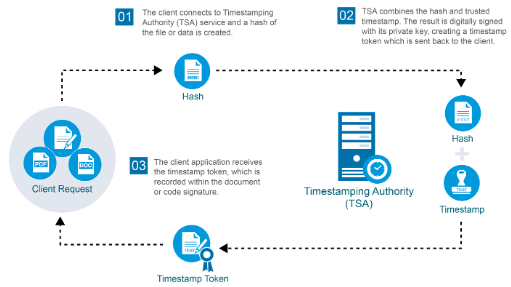
\includegraphics[scale=0.5]{TSA1.png}
\caption{Trusted Signature Architecture}
\label{fig:aesni_output_in_c}
\end{figure}

Thus we can conclude that Alice will be able to provide proof infront of the judge on when the file was created if she uses cryptographic signature..


\end{enumerate}



\section{Problem 3}

Suppose Alice and Bob store their respective RSA encryption public keys in a file on a server.
They communicate regularly using confidential messages. Eve wants to read the messages
but is unable to crack the RSA private keys of Alice and Bob. However, she is able to break into the server and alter the file containing Alice’s an Bob’s public keys.
\begin{enumerate}[label=\alph*]
\item \textbf{How should Eve alter that file so that she can read confidential messages sent between Alice and Bob and forge messages from either? After altering the file, how would she need to modify the communication to achieve the above?}

The main challenge that comes with public key encryption algorithms like RSA is to distribute the public key securely. We tend to share our public keys by electronic means such as emails, website and servers which poses a threat to the security of the key if the infrastructure is not trustworthy.\newline
The question above states this particular scenario, where the public key file is shared over a vulnerable server where Eve is able to break in. 
\begin{itemize}

\item Eve can replace the public key shared between Alice and Bob with her own public key(fake public key).

\item Thus when Alice sends a message to Bob, she will encrypt her message with Eve's public key and Eve will be able to decrypt them with her secret key.

\item Eve will now collect the data and encrypt it again with the original public key and send it to Bob.

\item Thus Bob will not able to understand if there has been an intrusion in the network and will assume that the message was sent by Alice.

\item This problem has led to lot of research in the practical cryptographic engineering and is the building block of Certificate Authority.

\end{itemize}

\item \textbf{How might Alice and/or Bob detect Eve’s subversion of the public keys?}

When a new message reaches Alice and/or Bob, they will not be able to identify if the message has been forged. Once the public keys of a network is compromised, there is nothing much to do in that scenario rather to protect the messages. Rather we can use new models for double layers of authentication.
To solve this problem Shamir has proposed a Key Generation Authority server that would create private keys. This is a slight modification on the previously proposed idea of generating public keys as unique identifiers. 
\begin{itemize}

\item At the time of setting up a trusted connection, the Key Generation Authority would generate a Master Public Key MPK which will be published and shared with everyone. 
\item If Alice wants to send a message to Bob, she will encrypt it using Bob's identifier and the MPK they have agreed to use. 
\item To decrypt the message Bob has to go to the Key Generation Authority and request for his secret key which is generated from the Master Secret Key MSK.
\end{itemize}
This Key Generation method would solve our above problem, albeit with a few drawbacks.

\begin{figure}[h!]
\centering
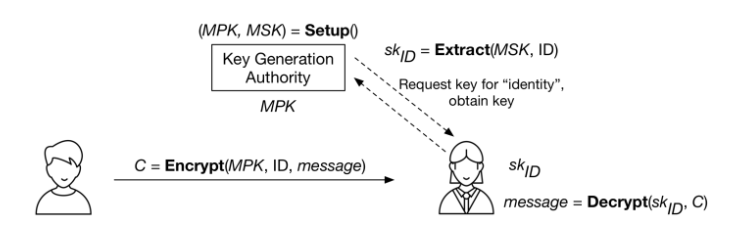
\includegraphics[scale=0.5]{key_generation_authority.png}
\caption{Identity Based Encryption System}
\label{fig:aesni_output_in_c}
\end{figure}

\end{enumerate}
\section{Problem 4}
Read the paper “Why Cryptosystems Fail” (available from
http://www.buffalo.edu/~mblanton/cse565/wcf.pdf) and answer the following questions
about it:
\begin{enumerate}[label=\alph*]
\item \textbf{What does the article tell you about security of computer systems and how the field of security evolves?}

The author dates back the convention the computer security designs were using to the 1970 conventional military wisdom. The time when ATMs were built it needed a cryptographic encryption system of the pin which adopted this expertise from the government sector.The military model stressed on the secrecy of the ATM pin and technical efforts, business and legal strategies were invested in achieving it. However the model proposed by the military world is an ideal scenario where the information will not be shared in a very controlled environment. When the banks tried to implement the same in the real world, the ATM pins secrecy was compromised  by crooks and even by the bank official. Some examples of the banks own security system are as follows:
\begin{itemize}

\item A technical staff in a bank in Scotland fitted the ATM with a hand held computer to record the customer's ATM pin and account numbers.

\item A well managed bank which implemented dual control over the unis-sued cards and ATM pins one day abolished the norm due to cost-cutting and the losses increased tenfold.

\item Another bank had implemented a system where telephone cards when inserted in an ATM machine, it believed that the previous ATM card was inserted again. This is a perfect example where an absurd programming error can lead to serious consequences.

\item A bank had implemented a method where the ATM pin was concealed on a squared cardboard which was designed to be kept along with the ATM card in the purse.Suppose your PIN is 2256. Choose a four-letter word, say ‘blue’. Write these four letters down in the second, second, fifth and sixth columns of the card respectively. The chances of getting the 4 digit ATM pin was 1/3333 which drastically reduced to 1/8 if stolen.

\begin{figure}[h!]
\centering
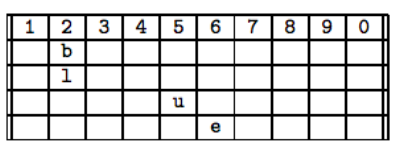
\includegraphics[scale=0.5]{Cardboard_pin.png}
\caption{Cardborad to represent ATM Pin}
\label{fig:aesni_output_in_c}
\end{figure}

\item A UK bank wrote the encrypted pin in the card strip. The criminal fraternity took 15 years to figure out that the account number on my card can be changed to someone else's account number to and use my own ATM pin to withdraw.\newline

Due to the above failures in security algorithm implementation, the standard approach that was adopted later on was called a security module which is a PC in a safe which manages all the keys and pins only in their encrypted form. Banks and ATM that belongs to the VISA and MASTERCARD atm networks used this security module. However this model failed as well when the system programmer could easily decrypt the ATM pin.

From the above examples, the author draws a line on how although there was evolution in the algorithms the banks used, no substantial progress could be made as long as the military model was followed.Thus he proposed the reductionist and holistic models as a better approach to look at security problems.




\end{itemize}


\item \textbf{What does it tell you about building and operating secure systems?}

While building a secure system from the article we can formulate the below things that needs to be considered for best results:

\begin{itemize}
\item Companies implementing security systems should hire better specialized software developers who would be able to implement the security algorithms without errors which would lead to extreme consequences. We had seen wrong implementations which lacked expertise in the case where telephone cards acted as debit cards when swiped in atms and changing account numbers on cards but using one's own pin to extract money.

\item Proper supervision by management in banks should be enforced to keep an eye on the clerks or technicians who have access to one's debit/credit cards and atm pins. Supervision must be enforced on software developers so that they do not have direct access to encrypt/decrypt the pins.

\item Banks that have been following well managed models like implementing dual control over unissued ATM cards and pins, cannot abolish secure systems and make it vulnerable just on the basis of cost. Cost is a factor we need to consider while building a secure system.

\item Critical information such as a person's account number as well as the ATM pin (in any form) should not be anywhere on the card. This increases the vulnerability of the pins as we had seen in the case of crooks collecting accounting numbers and forging blank cards to extract money.

\item We need experts both technicians and developers in the field of security who will have the expertise to implement the hardware versions of security products so that companies do not disregard it as a time-consuming and difficult to install machine like happened in the case of security module by VISA/MASTERCARD.

\item The security companies must provide their own trained and bonded personnel to
implement, maintain and manage the system.

\item We must automate tasks as suggested by Ross's mechanical model to avoid a third party interception to make the model less vulnerable.

\item We must implement systems which would follow an adaptive learning model to make the security system better with continuous improvement.

\end{itemize}

\item \textbf{What is the main proposal of the paper?}

The author Ross Anderson in this article points on how security designers and government evaluators have concentrated mostly on the technical weaknesses of the algorithm rather than on the implementation of it. For example the actual attacks that happened, were mostly due to the lack of expertise in this field resulting to system design errors, programming and administration errors. The authors points out that in the 1980's survey on the threat model , it was revealed , that the security designers mostly concentrated on speculating the probability of an event rather than the likeliness of it. The designers assumed that the attacker might have the expertise and technical tools as that of the government agencies to break into a system which was clearly not the case. So in this case, the threat model and an individual's ability to break into a system, was highly miscalculated.\newline

The author believes that since more and more people have become aware of the loopholes in the existing security systems, there is a need of rise of a new paradigm. The author suggests that instead of worrying on what might possible go wrong, we need to start a systematic study of what is likely to happen. When paradigm shift occurs, it is likely that we will import the model from an existing successful one which will give a base to our new emerging data.\newline

In the field of critical systems, the author has proposed two competing models -
\begin{itemize}
\item \textbf{Reductionist Model} - One example of a reductionist model is the Railway Signalling System, where the system is in control an the task of the driver of the train has been deskilled and been automated\newline

\item \textbf{Holistic Model} - An example where the Holistic model is implemented is the aviation system, where the control is in the hand of the pilot and improves incrementally on continuous feedback.\newline
\end{itemize}
\item \textbf{How do you think the situation with the banking industry today compares with what is described in the article?}

The banking industry in today's world varies drastically from what is described in the article in the year 1994. The security system has improved effectively over all these years with the emergence of internet and a plethora of new algorithms/procedures maintained by the banking system today. The reductionist model which Ross has suggested in him paper has been implemented in today's world with the automation of services in banking industry. 
\begin{itemize}
\item As the author mentioned one bank had an implementation that when money is withdrawn from the ATM and a statement is generated, that entry will not be displayed in a full statement that is generated at some later point in time. In contrast to this, we can generate statements anytime we want to from the ATM/bank/net banking nowadays by specifying the whole month as well as a particular time period and it will show records for every transaction made into the account.

\item Some banks used to print account numbers in the statements generated while withdrawal which could easily be forged by simple scams like observing customer pins. In today's world, account numbers are private information which is never displayed on debit cards, statements as well as on the net banking interface. 

\item Banks used to issue new cards whenever an update in withdrawal limit was requested by the customer through postal services along with the pins. This procedure has been completely disregarded in the modern day banking system where the cards are issued through post but we have to set our ATM pins by ourselves by calling the banking services and by passing a lot of verification procedures. For any updation in the account like card limit, the same card which was issues can be modified online by bank personals.  

\item Back in 1994, Italy's ATMs used to be an offline service and any amount we withdrew were not updated to the account immediately , but only in banking hours. However, with the rise of the world wide web, the ATMs are integrated with the internet for immediate updation to the account on any transaction whether made through atms or internet banking.

\item Any transaction/unexpected access/login over the internet banking as well as in the ATM in today's world are properly integrated with continuous alerts to our mail and telephone texts.These security alerts warns us of any unwanted access to our accounts. This was not available back in 1994 and customers had to rely on bank statements only.
\end{itemize}


\textbf{What are some of the protection mechanisms that you encountered in your banking experience?}

Banks have introduced several protection mechanisms nowadays to ensure banking security. Here is a list of them from my experience with banking:

\begin{itemize}
\item \textbf{Strong password and pass phrase support}
Online Banking systems urge customers to set long pass phrases such as `Turkey and stuFFing at 4599 Pet\$ Road`, which are difficult to crack using guessing or brute-force password attacks. 

\item \textbf{Risk-Based Authentication}
Banking systems provides RBA Risk Based Authentication through a number of security questions and security images. The purpose of using security images for authentication is to help customer identify a phishing site. A phishing site will not be able to display the correct security image for a user and thus we will avoid login in to netbanking in that case.

\item \textbf{Two-way Authentication Method}
Even when we login to the netbanking site with our credential and security image, for any transaction the bank will provide another layer of authentication i.e. it sends a passcode to the registered mail-id or phone number for double verification.

\item \textbf{Real-time Out-of-Band Transaction Alerts}
Banks/Credit union provides the user to configure deposit and withdrawal limits in their account, whenever an amount of value greater than the limit is withdrawn/deposited,a real-time notification is sent to our mail or phone.

\item \textbf{Self-ATM Pin Generation}
Banks avoid physically sending atm pins through postal services. However the card contains details to call the bank and generate your own atm pin , after a stream of authentication procedures.

\end{itemize}
\item \textbf{How do you think computer security in other industries compares to the security in the banking sector?}

Although banking and financial sectors are at the most risk of security attacks, there are other industries that are susceptible to security attacks as well:

\begin{itemize}
\item \textbf{HealthCare}
HealthCare industry has experienced one of the largest security breach in the year 2015 known as the Anthem Incident.It is an information intensive industry which has name, address, physical conditions information as well as financial details and thus is prone to attack. Compromised data in this case includes credit card information, social security number and employment information which cybercriminals can use to establish fake medical identities and performs phishing attacks on health online systems.Although the health industry invests in cybersecurity and uses tools like encryption, antivirus tools and firewalls, they need to replace outdated systems with newer ones.

\item \textbf{Manufacturing}
Manufacturing industries include automotive, electronic, textile, pharmaceutical good producers which hold critical research data which attacts cybercriminals towards this industry.They have a cache holding patents and business secrets.Robust cyber defence equipped systems are needed to protect this industry from cyber attacks. This sector has not yet fully realized the importance of cyber security making them a vulnerable field.

\item \textbf{Education}
The education institutions such as universities and colleges are targeted by cyber attackers because they produce high value research data and have high-end network infrastructure which help attackers to attack other sectors as well.By increasing awareness about potential threats of cyber attacks in university, cyber attacks can be controlled, because mostly attacks are through phishing emails or the university sites that students regularly visit.Data for 18,000 people were compromised in the cyber attacks in 2015.

\item \textbf{Government}
The Government sector is a hot favourite for cyber attacks because it consists of confidential data such as social security number, unique digital fingerprint. Government sectors have not yet built a strong cybersecurity system. Over 50 million Turkish residents were at a risk of identity theft when the government database was leaked.Government sectors should build FISMA based security management program and additional layers of protection for servers containing sensitive data.

Thus by comparing these sectors we can conclude that financial sector is the forerunner in implementing security systems.

\end{itemize}
\end{enumerate}

\bibliographystyle{plain}
\bibliography{references}
\begin{itemize}

\item Computer Security: Principles and Practice (3rd Edition), William Stallings; Lawrie Brown

\item Trusted Timestamps : https://www.globalsign.com/en/blog/what-is-timestamping-how-does-it-work/

\item Cipher Feedback : https://www.coursera.org/lecture/symmetric-crypto/cipher-feedback-cfb-7Irpe

\item Digital Signatures and Timestamp : https://www.sysadmins.lv/blog-en/digital-signatures.aspx

\item Beyond public key encryption : https://blog.cryptographyengineering.com/2017/07/02/beyond-public-key-encryption/

\item Security Tips for Banks to Protect Themselves and Customers Through Better Online Banking System  : https://www.inetsolution.com/blog/june-2011/security-tips-for-banks-to-protect-themselves-and

\item How top industries preparing for cyber security threats : https://www.globalsign.com/en/blog/top-industries-preparing-for-evolving-cybersecurity-threats/

\end{itemize}
\end{document}
